\begin{filecontents*}{references.bib}
@article{cheddad2010,
  author    = {Abbas Cheddad and Joan Condell and Kevin Curran and Paul McKevitt},
  title     = {Digital image steganography: Survey and analysis of current methods},
  journal   = {Signal Processing},
  volume    = {90},
  number    = {3},
  pages     = {727--752},
  year      = {2010},
  doi       = {10.1016/j.sigpro.2009.08.010}
}

@book{cox2007,
  author    = {Ingemar J. Cox and Matthew L. Miller and Jeffrey A. Bloom and Jessica Fridrich and Ton Kalker},
  title     = {Digital Watermarking and Steganography},
  publisher = {Morgan Kaufmann},
  edition   = {2},
  year      = {2007}
}

@book{fridrich2009book,
  author    = {Jessica Fridrich},
  title     = {Steganography in Digital Media: Principles, Algorithms, and Applications},
  publisher = {Cambridge University Press},
  year      = {2009}
}

@article{bender1996,
  author    = {Walter Bender and Daniel Gruhl and Norishige Morimoto and Anthony Lu},
  title     = {Techniques for data hiding},
  journal   = {IBM Systems Journal},
  volume    = {35},
  number    = {3--4},
  pages     = {313--336},
  year      = {1996},
  doi       = {10.1147/sj.353.0313}
}

@article{chan2004,
  author    = {Chi-Kwong Chan and L. M. Cheng},
  title     = {Hiding data in images by simple {LSB} substitution},
  journal   = {Pattern Recognition},
  volume    = {37},
  number    = {3},
  pages     = {469--474},
  year      = {2004},
  doi       = {10.1016/j.patcog.2003.08.007}
}

@article{wu2003,
  author    = {Da-Chun Wu and Wen-Hsiang Tsai},
  title     = {A steganographic method for images by pixel-value differencing},
  journal   = {Pattern Recognition Letters},
  volume    = {24},
  number    = {9--10},
  pages     = {1613--1626},
  year      = {2003},
  doi       = {10.1016/S0167-8655(02)00402-6}
}

@inproceedings{westfeld1999,
  author    = {Andreas Westfeld and Andreas Pfitzmann},
  title     = {Attacks on steganographic systems},
  booktitle = {Information Hiding},
  series    = {Lecture Notes in Computer Science},
  volume    = {1768},
  pages     = {61--76},
  publisher = {Springer},
  year      = {1999}
}

@inproceedings{fridrich2001,
  author    = {Jessica Fridrich and Miroslav Goljan and Rui Du},
  title     = {Reliable detection of {LSB} steganography in color and grayscale images},
  booktitle = {Proceedings of the ACM Workshop on Multimedia and Security},
  pages     = {27--30},
  year      = {2001},
  doi       = {10.1145/1232454.1232469}
}

@article{dumitrescu2003,
  author    = {Sorin Dumitrescu and Xiaolin Wu and Zhe Wang},
  title     = {Detection of {LSB} steganography via sample pair analysis},
  journal   = {IEEE Transactions on Signal Processing},
  volume    = {51},
  number    = {7},
  pages     = {1995--2007},
  year      = {2003},
  doi       = {10.1109/TSP.2003.812753}
}

@article{pevny2010,
  author    = {Tom{\'a}{\v{s}} Pevn{\'y} and Tom{\'a}{\v{s}} Filler and Patrick Bas},
  title     = {Using high-dimensional image models to perform highly undetectable steganography},
  journal   = {Information Hiding},
  volume    = {6387},
  pages     = {161--177},
  year      = {2010}
}

@article{filler2011,
  author    = {Tom{\'a}{\v{s}} Filler and Jan Judas and Jessica Fridrich},
  title     = {Minimizing additive distortion in steganography using syndrome-trellis codes},
  journal   = {IEEE Transactions on Information Forensics and Security},
  volume    = {6},
  number    = {3},
  pages     = {920--935},
  year      = {2011},
  doi       = {10.1109/TIFS.2011.2134094}
}

@inproceedings{holub2012,
  author    = {Vojt{\v{e}}ch Holub and Jessica Fridrich},
  title     = {Designing steganographic distortion using directional filters},
  booktitle = {Proceedings of IEEE International Workshop on Information Forensics and Security},
  pages     = {234--239},
  year      = {2012},
  doi       = {10.1109/WIFS.2012.6412655}
}

@article{holub2014,
  author    = {Vojt{\v{e}}ch Holub and Jessica Fridrich and Tom{\'a}{\v{s}} Denemark},
  title     = {Universal distortion function for steganography in an arbitrary domain},
  journal   = {EURASIP Journal on Information Security},
  volume    = {2014},
  number    = {1},
  pages     = {1},
  year      = {2014},
  doi       = {10.1186/1687-417X-2014-1}
}

@article{fridrich2012rich,
  author    = {Jessica Fridrich and Jan Kodovsk{\'y}},
  title     = {Rich models for steganalysis of digital images},
  journal   = {IEEE Transactions on Information Forensics and Security},
  volume    = {7},
  number    = {3},
  pages     = {868--882},
  year      = {2012},
  doi       = {10.1109/TIFS.2012.2190402}
}

@article{kodovsky2012ensemble,
  author    = {Jan Kodovsk{\'y} and Jessica Fridrich and Vojt{\v{e}}ch Holub},
  title     = {Ensemble classifiers for steganalysis of digital media},
  journal   = {IEEE Transactions on Information Forensics and Security},
  volume    = {7},
  number    = {2},
  pages     = {432--444},
  year      = {2012},
  doi       = {10.1109/TIFS.2011.2175919}
}

@inproceedings{hidden2018,
  author    = {Jiren Zhu and Russell Kaplan and Justin Johnson and Li Fei-Fei},
  title     = {{HiDDeN}: Hiding data with deep networks},
  booktitle = {Proceedings of the European Conference on Computer Vision},
  pages     = {657--672},
  year      = {2018}
}

@article{yedroudj2018,
  author    = {Mounir Yedroudj and Fr{\'e}d{\'e}ric Comby and Marc Chaumont},
  title     = {{Yedroudj-Net}: An efficient {CNN} for spatial steganalysis},
  journal   = {Proceedings of ICASSP},
  pages     = {2092--2096},
  year      = {2018},
  doi       = {10.1109/ICASSP.2018.8461438}
}

@article{boroumand2019,
  author    = {Masoud Boroumand and Mo Chen and Jessica Fridrich},
  title     = {Deep residual network for steganalysis of digital images},
  journal   = {IEEE Transactions on Information Forensics and Security},
  volume    = {14},
  number    = {5},
  pages     = {1181--1193},
  year      = {2019},
  doi       = {10.1109/TIFS.2018.2871749}
}

@article{khurshid2020,
  author    = {Farhana Khurshid and A. H. Mir},
  title     = {Fuzzy logic-based adaptive image steganography for secure digital communication},
  journal   = {Multimedia Tools and Applications},
  volume    = {79},
  pages     = {26777--26798},
  year      = {2020},
  doi       = {10.1007/s11042-020-09203-z}
}

@inproceedings{abdulla2014,
  author    = {A. A. Abdulla and H. Sellahewa and S. A. Jassim},
  title     = {Steganography based on pixel intensity value decomposition},
  booktitle = {SPIE Mobile Multimedia/Image Processing, Security, and Applications},
  year      = {2014}
}

@article{hussain2018,
  author    = {Mehdi Hussain and Ainuddin Wahid Abdul Wahab and Yamani Idna Bin Idris and Anthony T. S. Ho and Ki-Hyun Jung},
  title     = {Image steganography in spatial domain: A survey},
  journal   = {Signal Processing: Image Communication},
  volume    = {65},
  pages     = {46--66},
  year      = {2018},
  doi       = {10.1016/j.image.2018.03.012}
}

@article{survey2022,
  author    = {S. Alanazi and A. M. Aljuaid and M. N. Khan and others},
  title     = {Digital image steganography survey and investigation: Goal, assessment, method, development, and dataset},
  journal   = {Signal Processing},
  volume    = {199},
  pages     = {108617},
  year      = {2022}
}

@article{systematic2024,
  author    = {A. B. Ogundokun and O. A. Arulogun and others},
  title     = {Image steganography techniques for resisting statistical steganalysis attacks: A systematic literature review},
  journal   = {PLOS ONE},
  volume    = {19},
  number    = {9},
  pages     = {e0308807},
  year      = {2024}
}

@article{zadeh1965,
  author    = {Lotfi A. Zadeh},
  title     = {Fuzzy sets},
  journal   = {Information and Control},
  volume    = {8},
  number    = {3},
  pages     = {338--353},
  year      = {1965},
  doi       = {10.1016/S0019-9958(65)90241-X}
}

@article{mamdani1975,
  author    = {Ebrahim H. Mamdani and Sedrak Assilian},
  title     = {An experiment in linguistic synthesis with a fuzzy logic controller},
  journal   = {International Journal of Man-Machine Studies},
  volume    = {7},
  number    = {1},
  pages     = {1--13},
  year      = {1975},
  doi       = {10.1016/S0020-7373(75)80002-2}
}

@book{ross2010,
  author    = {Timothy J. Ross},
  title     = {Fuzzy Logic with Engineering Applications},
  publisher = {Wiley},
  edition   = {3},
  year      = {2010}
}

@article{wang1992,
  author    = {Li-Xin Wang and Jerry M. Mendel},
  title     = {Generating fuzzy rules by learning from examples},
  journal   = {IEEE Transactions on Systems, Man, and Cybernetics},
  volume    = {22},
  number    = {6},
  pages     = {1414--1427},
  year      = {1992},
  doi       = {10.1109/21.199466}
}

@article{shannon1948,
  author    = {Claude E. Shannon},
  title     = {A mathematical theory of communication},
  journal   = {Bell System Technical Journal},
  volume    = {27},
  number    = {3},
  pages     = {379--423},
  year      = {1948},
  doi       = {10.1002/j.1538-7305.1948.tb01338.x}
}

@article{wang2004,
  author    = {Zhou Wang and Alan C. Bovik and Hamid R. Sheikh and Eero P. Simoncelli},
  title     = {Image quality assessment: From error visibility to structural similarity},
  journal   = {IEEE Transactions on Image Processing},
  volume    = {13},
  number    = {4},
  pages     = {600--612},
  year      = {2004},
  doi       = {10.1109/TIP.2003.819861}
}

@misc{rfc9106,
  author       = {{IRTF CFRG}},
  title        = {{RFC 9106}: Argon2 Memory-Hard Function for Password Hashing and Proof-of-Work Applications},
  year         = {2021},
  howpublished = {\url{https://www.rfc-editor.org/rfc/rfc9106}}
}

@misc{nistgcm,
  author       = {{National Institute of Standards and Technology}},
  title        = {{NIST SP 800-38D}: Recommendation for Block Cipher Modes of Operation: Galois/Counter Mode (GCM) and GMAC},
  year         = {2007},
  howpublished = {\url{https://csrc.nist.gov/publications/detail/sp/800-38d/final}}
}

@article{zhang2011,
  author    = {Xinpeng Zhang},
  title     = {Reversible data hiding in encrypted images},
  journal   = {IEEE Signal Processing Letters},
  volume    = {18},
  number    = {4},
  pages     = {255--258},
  year      = {2011},
  doi       = {10.1109/LSP.2011.2114651}
}

@inproceedings{filler2010,
  author    = {Tom{\'a}{\v{s}} Filler and Jan Judas and Jessica Fridrich},
  title     = {Minimizing embedding impact in steganography using trellis-coded quantization},
  booktitle = {SPIE Media Forensics and Security},
  volume    = {7541},
  year      = {2010}
}

@inproceedings{bas2011boss,
  author    = {Patrick Bas and Tom{\'a}{\v{s}} Filler and Tom{\'a}{\v{s}} Pevn{\'y}},
  title     = {Break our steganographic system: The ins and outs of organizing {BOSS}},
  booktitle = {Information Hiding},
  pages     = {59--70},
  publisher = {Springer},
  year      = {2011}
}

@misc{bows2007,
  author       = {Patrick Bas and Teddy Furon},
  title        = {{BOWS-2} contest},
  year         = {2007},
  howpublished = {\url{http://bows2.ec-lille.fr}}
}

@article{ker2013,
  author    = {Andrew D. Ker and Tom{\'a}{\v{s}} Pevn{\'y} and Jessica Fridrich and Patrick Bas},
  title     = {Moving steganography and steganalysis from the laboratory into the real world},
  journal   = {Proceedings of the 1st ACM Workshop on Information Hiding and Multimedia Security},
  pages     = {45--58},
  year      = {2013}
}

@article{denemark2015,
  author    = {Tom{\'a}{\v{s}} Denemark and Jan Kodovsk{\'y} and Jessica Fridrich},
  title     = {Steganalysis features for content-adaptive {JPEG} steganography},
  journal   = {IEEE Transactions on Information Forensics and Security},
  volume    = {10},
  number    = {8},
  pages     = {1736--1746},
  year      = {2015}
}

@article{alrusaini2025,
  author    = {O. A. Alrusaini and others},
  title     = {Deep learning for steganalysis: Evaluating model robustness under image transformations},
  journal   = {Frontiers in Artificial Intelligence},
  volume    = {8},
  pages     = {1532895},
  year      = {2025}
}

@inproceedings{huiskes2008,
  author    = {Mark J. Huiskes and Michael S. Lew},
  title     = {The {MIR} {Flickr} retrieval evaluation},
  booktitle = {Proceedings of the 1st ACM International Conference on Multimedia Information Retrieval},
  pages     = {39--43},
  year      = {2008},
  doi       = {10.1145/1460096.1460104}
}
\end{filecontents*}

\documentclass[preprint,12pt]{elsarticle}

\usepackage{amssymb}
\usepackage{amsmath}
\usepackage{booktabs}
\usepackage{multirow}
\usepackage{array}
\usepackage{graphicx}
\usepackage{subcaption}
\usepackage{algorithm}
\usepackage{algpseudocode}
\usepackage{float}
\usepackage{adjustbox}
\usepackage{longtable}
\usepackage{url}
\usepackage{hyperref}
\usepackage{enumitem}
\usepackage{placeins}
\usepackage{xcolor}

\journal{Journal of Information Security and Applications}

\newcommand{\safeincludegraphics}[3]{%
\IfFileExists{#1}{\includegraphics[#2]{#1}}{%
\fbox{\parbox[c][5cm][c]{0.85\linewidth}{\centering #3\\[4pt]\texttt{#1}}}}%
}

\newcommand{\safesubimage}[2]{%
\IfFileExists{#1}{\includegraphics[width=\linewidth]{#1}}{%
\fbox{\parbox[c][2.8cm][c]{0.92\linewidth}{\centering #2\\[2pt]\scriptsize\texttt{#1}}}}%
}

\begin{document}

\begin{frontmatter}

\title{Adaptive Fuzzy Logic-Based Steganographic Encryption Framework: A Comprehensive Experimental Evaluation}

\author[inst1]{Aadi Joshi\corref{cor1}}
\ead{toaadijoshi@gmail.com}

\author[inst1]{Kavya Bhand}
\ead{kavya.bhand0806@gmail.com}


\cortext[cor1]{Corresponding author}

\affiliation[inst1]{
  organization={Vishwakarma Institute of Technology},
  city={Pune},
  state={Maharashtra},
  country={India}
}

\begin{abstract}
Digital image steganography requires a careful trade-off among payload capacity, visual fidelity, and statistical undetectability. Fixed-depth least significant bit embedding remains attractive because of its simplicity and high capacity, but it modifies smooth and textured regions uniformly, thereby increasing distortion and detectability in statistically sensitive areas. This paper presents an adaptive steganographic framework that combines a Mamdani-type fuzzy inference system with modern authenticated encryption. The proposed method determines a pixel-wise embedding depth from 1 to 3 bits using local entropy, edge magnitude, and payload pressure as linguistic inputs. To preserve encoder-decoder synchronization, the same feature maps are computed from lower-bit-stripped images, making the adaptive control mechanism invariant to the least significant modifications introduced during embedding. A cryptographic layer based on Argon2id and AES-256-GCM protects payload confidentiality and integrity independently of steganographic concealment.

The framework is evaluated on a synthetic corpus of 1,000 RGB images (\(256 \times 256\)) across five payload levels from 0.05 to 0.40 bpp, using fixed LSB-1 and fixed LSB-2 as baselines. To confirm cross-dataset generalizability, the same protocol is applied to three established steganography benchmarks: BOSSBase 1.01 and BOWS2 (512\(\times\)512 PGM, 200 images each) and MIRFLICKR (256\(\times\)256 JPEG, 200 images). The evaluation includes PSNR, SSIM, MSE, KL divergence, RS analysis, chi-square attack, sample pair analysis, paired \(t\)-tests with Bonferroni correction, Cohen's \(d\) effect sizes, confidence intervals, power analysis, feature-based steganalysis using SRM-lite with Fisher LDA, ablation studies, synchronization validation, extraction-success validation, and computational overhead profiling.

The adaptive approach consistently achieves approximately 3 dB PSNR advantage over Fixed-LSB-1 and approximately 7 dB over Fixed-LSB-2 across all four tested datasets, demonstrating that this quality benefit is stable under diverse image content. On MIRFLICKR, the adaptive method achieves a SRM-lite AUC of 0.565 at 0.05 bpp --- practically indistinguishable from a random classifier (AUC~=~0.5) --- representing the strongest steganalytic evasion result across all datasets. The results demonstrate that fuzzy depth control is an effective and interpretable mechanism for improving the quality-security trade-off in spatial-domain steganography, while also clarifying the limitations of adaptive LSB designs against stronger modern steganalysis.
\end{abstract}

\begin{keyword}
Image steganography \sep Fuzzy logic \sep Adaptive embedding \sep Least significant bit \sep Steganalysis \sep Argon2id \sep AES-GCM \sep Image security \sep BOSSBase \sep BOWS2 \sep MIRFLICKR
\end{keyword}

\end{frontmatter}

\section{Introduction}
Steganography aims to hide the existence of communication by embedding a message inside an apparently innocent carrier, whereas cryptography protects message content but does not conceal the presence of communication itself \cite{cheddad2010,cox2007,fridrich2009book}. In digital imagery, least significant bit replacement remains one of the most widely studied spatial-domain steganographic techniques because it is simple, computationally lightweight, and capable of high embedding capacity \cite{bender1996,chan2004,hussain2018}. However, fixed-depth LSB embedding treats all image regions identically, even though smooth, edge-dominant, and textured areas differ substantially in their perceptual masking behavior and their susceptibility to statistical steganalysis \cite{westfeld1999,fridrich2001,dumitrescu2003}. As a result, the same payload depth that is visually tolerable in a complex region may be highly conspicuous in a smooth region.

The broader steganographic literature has responded to this problem through content-adaptive and distortion-minimization frameworks such as HUGO, WOW, and S-UNIWARD \cite{pevny2010,filler2011,holub2012,holub2014}. These methods are conceptually strong and often more secure than simple LSB replacement, but they generally depend on more complex cost functions, coding strategies, and optimization procedures. By contrast, fuzzy logic offers an interpretable alternative for adaptive decision making under uncertainty \cite{zadeh1965,mamdani1975,ross2010}. Image complexity is rarely partitioned by crisp thresholds, and linguistic rules such as low entropy, medium edge strength, or high capacity pressure are natural descriptors for embedding decisions.

This work proposes an adaptive fuzzy logic-based steganographic framework with four design goals. First, it uses entropy and edge features extracted from lower-bit-stripped images so that the encoder and decoder compute identical adaptive maps. Second, it employs a Mamdani fuzzy inference engine with 27 rules to assign pixel-wise LSB depth in the range 1 to 3 bits. Third, it integrates modern payload protection through Argon2id key derivation and AES-256-GCM authenticated encryption \cite{rfc9106,nistgcm}. Fourth, it evaluates the approach at scale using 1,000 images on a synthetic corpus and 200 images each from three real-world benchmarks (BOSSBase 1.01, BOWS2, MIRFLICKR), with five embedding rates, paired statistical tests, feature-based steganalysis, ablations, synchronization validation, and complexity analysis.

The principal contributions of the paper are as follows:
\begin{enumerate}[leftmargin=1.2cm]
    \item An adaptive LSB steganographic framework that uses interpretable fuzzy rules to allocate embedding depth according to local entropy, edge structure, and payload pressure.
    \item An LSB-invariant feature extraction strategy that stabilizes encoder-decoder synchronization by stripping the lower 3 bits prior to grayscale conversion and local analysis.
    \item Integration of Argon2id and AES-256-GCM to separate steganographic concealment from cryptographic confidentiality and integrity \cite{rfc9106,nistgcm}.
    \item A comprehensive experimental evaluation with fidelity metrics, classical steganalysis, feature-based detection, statistical significance testing, ablation studies, synchronization analysis, and computational profiling.
    \item Validation on three real-world steganography benchmarks (BOSSBase 1.01, BOWS2, MIRFLICKR) confirming cross-dataset generalizability of quality gains and steganalysis improvements \cite{bas2011boss,bows2007,huiskes2008}.
\end{enumerate}

The paper is deliberately conservative in its claims. The proposed system improves image quality substantially and improves detector behavior relative to fixed LSB baselines at multiple payloads, but it does not claim superiority over modern distortion-minimization algorithms or deep-learning steganalyzers \cite{fridrich2012rich,kodovsky2012ensemble,yedroudj2018,boroumand2019,alrusaini2025}.

\section{Related Work}
\subsection{Classical LSB steganography}
Early spatial steganography emphasized direct least significant bit replacement because it offered a practical route to high-capacity embedding with minimal algorithmic complexity \cite{bender1996,fridrich2009book}. This convenience, however, came at the cost of detectable statistical artifacts. Westfeld and Pfitzmann showed that LSB modifications alter pairs-of-values distributions in ways exploitable by chi-square analysis \cite{westfeld1999}. Fridrich et al.\ introduced RS analysis, which remains one of the canonical detectors for spatial LSB steganography \cite{fridrich2001}. Dumitrescu et al.\ further developed sample pair analysis to estimate hidden payload characteristics from adjacent sample statistics \cite{dumitrescu2003}. These attacks collectively established that naively uniform embedding is statistically fragile.

\subsection{Adaptive and distortion-based embedding}
The next major progression in steganography involved assigning different embedding risks to different image components. HUGO used high-dimensional image modeling to design highly undetectable embedding costs \cite{pevny2010}. Syndrome-trellis codes then provided an efficient coding framework for minimizing additive distortion under such cost maps \cite{filler2011,filler2010}. WOW introduced directional filters to identify embedding locations that would be less detectable by steganalysis \cite{holub2012}, while S-UNIWARD generalized the distortion-function perspective to arbitrary domains \cite{holub2014}. These approaches offer stronger theoretical underpinnings than conventional LSB replacement and represent a higher security baseline for spatial steganography.

\subsection{Steganalysis}
Steganalysis has evolved from hand-crafted statistical attacks to rich-model and deep-learning paradigms. Rich models capture dependencies in high-pass residuals and have produced strong universal detectors for both spatial and transform-domain embedding \cite{fridrich2012rich,kodovsky2012ensemble,denemark2015}. More recently, convolutional neural networks such as Yedroudj-Net and deep residual architectures such as SRNet have further improved performance by learning discriminative residual features end-to-end \cite{yedroudj2018,boroumand2019}. Recent reviews indicate that robust evaluation of any steganographic scheme should consider this broader detection landscape, especially under transformations and dataset mismatch \cite{systematic2024,alrusaini2025}.

\subsection{Fuzzy logic and cryptographic integration}
Fuzzy logic has long been used for inference under ambiguity and gradual transitions \cite{zadeh1965,mamdani1975,ross2010,wang1992}. In image security, fuzzy reasoning has been applied to adaptive embedding decisions, capacity allocation, and pixel selection, although prior work often used simpler rules or less extensive security analysis \cite{khurshid2020,abdulla2014}. In parallel, secure steganographic systems increasingly combine concealment with encryption, recognizing that covert transport alone is insufficient if the payload can be recovered after detection \cite{cox2007,zhang2011}. Current best practice favors memory-hard password derivation and authenticated encryption rather than unauthenticated block-cipher modes \cite{rfc9106,nistgcm}. The present work unifies these ideas in a single experimentally grounded framework.

\section{Proposed Framework}
\subsection{Notation and problem definition}
Let the cover image be \(I_c \in \{0,\ldots,255\}^{H \times W \times C}\), where \(H\), \(W\), and \(C\) denote height, width, and channel count. The goal is to embed a protected payload into \(I_c\) to produce a stego image \(I_s\), while maximizing visual fidelity and minimizing statistical detectability. Unlike fixed schemes that embed a constant number of bits per sample, the proposed method learns a depth map \(D(x,y) \in \{1,2,3\}\) that adapts to local content.

\subsection{System overview}
Figure~\ref{fig:architecture} summarizes the full encoder-decoder pipeline. The encoder computes local entropy and edge magnitude from an LSB-invariant image representation, combines those with payload pressure in a Mamdani fuzzy inference system, encrypts the payload using Argon2id and AES-256-GCM, and writes bits in a pseudo-random order according to the adaptive depth map. The decoder reconstructs the same feature maps and depth map from the stego image, extracts the ciphertext in the same order, and decrypts it without explicitly transmitting the depth map.

\begin{figure}[H]
    \centering
    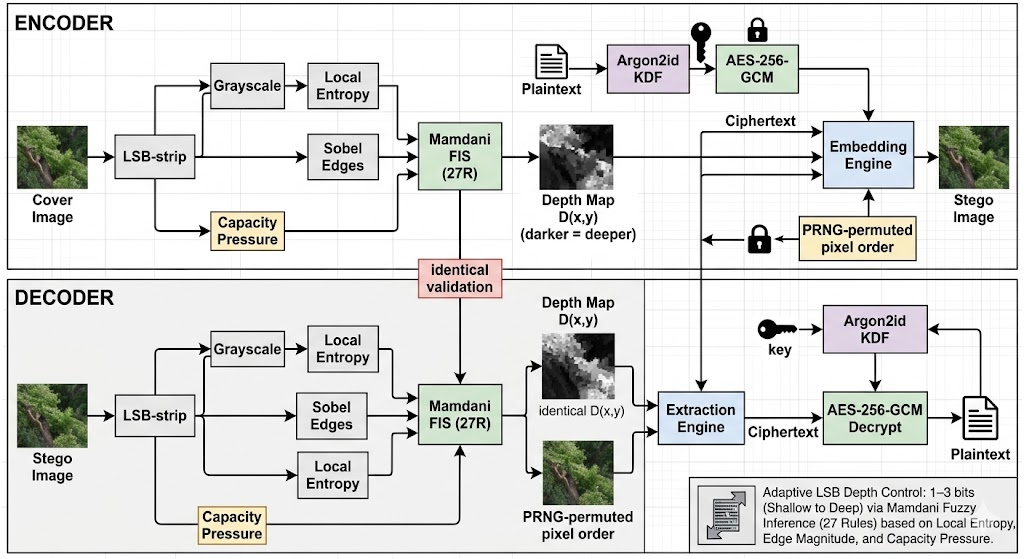
\includegraphics[width=0.96\linewidth]{architecture.jpeg}
    \caption{Overall architecture of the adaptive fuzzy logic-based steganographic encryption framework. The depth map is not transmitted; instead, it is reconstructed deterministically by both encoder and decoder from LSB-invariant feature extraction.}
    \label{fig:architecture}
\end{figure}

\subsection{LSB-invariant feature extraction}
A critical challenge in adaptive steganography is synchronization. If the encoder selects embedding depths from the cover image but the decoder recomputes those depths from the stego image, even small LSB perturbations can cause a mismatch. To avoid this, features are computed from a lower-bit-stripped representation:
\begin{equation}
I_{\text{strip}}(x,y,c)=I(x,y,c)\wedge \texttt{0xF8}.
\end{equation}
The grayscale image used for analysis is then
\begin{equation}
G(x,y)=0.299\,I_{\text{strip}}(x,y,R)+0.587\,I_{\text{strip}}(x,y,G)+0.114\,I_{\text{strip}}(x,y,B).
\end{equation}

Local Shannon entropy within a window \(\Omega_{x,y}\) is defined as
\begin{equation}
H(x,y)=-\sum_{b=0}^{63} p_b(x,y)\log_2 p_b(x,y),
\end{equation}
where \(p_b(x,y)\) is the local probability of intensity bin \(b\) \cite{shannon1948}. Edge magnitude is computed using Sobel operators:
\begin{equation}
E(x,y)=\frac{\sqrt{(G*S_x)^2+(G*S_y)^2}}{\max_{(x',y')}\sqrt{(G*S_x)^2+(G*S_y)^2}}.
\end{equation}
This normalization maps the edge descriptor to \([0,1]\). Together, \(H\) and \(E\) capture statistical complexity and local masking conditions while remaining stable under the 1 to 3-bit LSB modifications introduced by the embedding stage.

\subsection{Fuzzy inference system}
The adaptive controller is a Mamdani fuzzy inference system with three inputs:
\begin{itemize}[leftmargin=0.9cm]
    \item Entropy \(H\), with linguistic labels Low, Medium, and High.
    \item Edge magnitude \(E\), with linguistic labels Low, Medium, and High.
    \item Capacity pressure \(P\), with linguistic labels Low, Medium, and High.
\end{itemize}
The output is embedding depth \(D\), represented by the fuzzy sets Shallow, Moderate, and Deep over the interval \([1,3]\).

All variables use trapezoidal membership functions:
\begin{equation}
\mu(x;a,b,c,d)=\max\left(\min\left(\frac{x-a}{b-a},1,\frac{d-x}{d-c}\right),0\right).
\end{equation}
The complete system contains \(3 \times 3 \times 3 = 27\) rules. These rules encode the intuitive principle that deeper embedding is more permissible in high-entropy, high-edge regions, while payload pressure modulates how aggressively the method consumes available capacity.

Representative rules include:
\begin{enumerate}[leftmargin=1.2cm]
    \item If entropy is Low, edge is Low, and pressure is Low, then depth is Shallow.
    \item If entropy is Medium, edge is Medium, and pressure is Medium, then depth is Moderate.
    \item If entropy is High, edge is High, and pressure is High, then depth is Deep.
\end{enumerate}

Rule firing uses the Mamdani minimum \(t\)-norm:
\begin{equation}
\alpha_r=\min\left(\mu_{H_r}(H),\mu_{E_r}(E),\mu_{P_r}(P)\right).
\end{equation}
Aggregation across output sets uses the maximum \(s\)-norm, and centroid defuzzification yields
\begin{equation}
D^*(x,y)=\frac{\int d \cdot \mu_{\text{agg}}(d)\,dd}{\int \mu_{\text{agg}}(d)\,dd}.
\end{equation}
The operational depth is then \(D(x,y)=\mathrm{clip}(\lfloor D^*(x,y)+0.5 \rfloor,1,3)\).

\subsection{Adaptive capacity and embedding}
Given the depth map \(D(x,y)\) and channel count \(C\), adaptive capacity per pixel is
\begin{equation}
\mathrm{Cap}(x,y)=D(x,y)\cdot C \text{ bits}.
\end{equation}
Total capacity is \(\sum_{x,y}\mathrm{Cap}(x,y)\). Embedding proceeds in pseudo-random order using a key-dependent permutation. For each selected sample, the algorithm writes a number of payload bits equal to the local depth value. This heterogeneous assignment protects smooth areas while allowing deeper embedding in more permissive regions.

\subsection{Cryptographic layer}
The payload is encrypted before embedding. A 256-bit key is derived using Argon2id:
\begin{equation}
K=\mathrm{Argon2id}(\text{password},\sigma,t=3,m=64\,\text{MiB},p=4),
\end{equation}
where \(\sigma\) is a randomly generated salt \cite{rfc9106}. Authenticated encryption is then performed using AES-256-GCM:
\begin{equation}
(\hat{m},\tau)=\mathrm{AES\mbox{-}GCM}_{K}(\nu,m),
\end{equation}
where \(\nu\) is a fresh nonce and \(\tau\) is the authentication tag \cite{nistgcm}. The embedded wire format is \(\sigma \Vert \nu \Vert \hat{m} \Vert \tau\). This design ensures confidentiality and integrity even if covert transport is compromised.

\subsection{Algorithms}
\begin{algorithm}[H]
\caption{Adaptive fuzzy embedding}
\begin{algorithmic}[1]
\Require Cover image \(I_c\), plaintext message \(m\), password, seed
\Ensure Stego image \(I_s\)
\State Generate random salt \(\sigma\)
\State Derive \(K \gets \mathrm{Argon2id}(\text{password},\sigma)\)
\State Generate random nonce \(\nu\)
\State Encrypt \(m\) with AES-256-GCM to obtain \(\hat{m}\) and tag \(\tau\)
\State Form payload \(W=\sigma \Vert \nu \Vert \hat{m} \Vert \tau\)
\State Compute \(I_{\text{strip}}\), grayscale image, entropy map \(H\), and edge map \(E\)
\State Estimate payload pressure \(P\) from message length and adaptive capacity
\ForAll{pixels \((x,y)\)}
    \State Fuzzify \(H(x,y)\), \(E(x,y)\), and \(P\)
    \State Evaluate the 27 fuzzy rules
    \State Defuzzify and quantize to obtain \(D(x,y)\in\{1,2,3\}\)
\EndFor
\State Generate pseudo-random sample order \(\pi\)
\State Embed the bitstream in permuted order using local depth \(D(x,y)\)
\State \Return \(I_s\)
\end{algorithmic}
\end{algorithm}

\begin{algorithm}[H]
\caption{Adaptive extraction}
\begin{algorithmic}[1]
\Require Stego image \(I_s\), password, seed
\Ensure Recovered message \(m\) or failure \(\bot\)
\State Recompute \(I_{\text{strip}}\), entropy map, edge map, and depth map
\State Regenerate pseudo-random sample order \(\pi\)
\State Extract header and payload bits according to \(D(x,y)\)
\State Parse \(\sigma \Vert \nu \Vert \hat{m} \Vert \tau\)
\State Derive \(K \gets \mathrm{Argon2id}(\text{password},\sigma)\)
\State Attempt AES-256-GCM decryption and authentication
\If{verification fails}
    \State \Return \(\bot\)
\Else
    \State \Return \(m\)
\EndIf
\end{algorithmic}
\end{algorithm}

\section{Threat Model}
The threat model follows a cover-free setting in which the adversary has access to the stego image but not the original cover \cite{fridrich2009book,ker2013}. Three classes of adversaries are considered.

\textbf{Passive steganalyst.} This adversary applies statistical or learned detectors, including RS analysis, chi-square analysis, sample pair analysis, and rich-model or neural steganalyzers, to determine whether hidden information is present \cite{westfeld1999,fridrich2001,dumitrescu2003,fridrich2012rich,kodovsky2012ensemble,yedroudj2018,boroumand2019}.

\textbf{Active attacker.} This adversary modifies the image through cropping, noise injection, resizing, or compression in an attempt to corrupt the embedded payload.

\textbf{Cryptanalytic adversary.} This adversary gains access to the extracted ciphertext and attempts password guessing, nonce misuse exploitation, or ciphertext tampering.

The system targets improved undetectability relative to fixed LSB, not perfect covertness. Confidentiality and integrity rely on standard assumptions for Argon2id and AES-GCM \cite{rfc9106,nistgcm}. The framework does not claim robustness against lossy operations, which are fundamentally problematic for spatial LSB methods \cite{cheddad2010,hussain2018}. It also does not claim resistance to the strongest modern deep-learning steganalyzers.

\section{Experimental Setup}
\subsection{Synthetic dataset}
The framework is initially evaluated on 1,000 RGB images of size \(256 \times 256\), generated to span five texture categories with distinct entropy and edge characteristics: smooth, noise, natural-like, textured, and mixed. Each category contains 200 samples. The smooth class contains gradient and blurred content; the noise class contains random patterns; the natural-like class uses \(1/f\) spectral statistics; the textured class includes sinusoidal and Gabor-like patterns; and the mixed class combines multiple local regimes. A fixed random seed of 42 is used for reproducibility.

This controlled design provides broad structural diversity for evaluating adaptive feature-based embedding. Conclusions from the synthetic corpus are framed around internal comparative validity, with cross-dataset generalizability confirmed separately on real-world benchmarks (Section~\ref{sec:real_datasets}).

\begin{table}[H]
\centering
\caption{Synthetic dataset composition}
\label{tab:dataset}
\begin{tabular}{lccc}
\toprule
Category & Count & Entropy range & Description \\
\midrule
Smooth & 200 & 1--3 bits & Gradient + Gaussian blur \\
Noise & 200 & 6--8 bits & Random pixel patterns \\
Natural-like & 200 & 4--6 bits & 1/f spectral noise \\
Textured & 200 & 5--7 bits & Sinusoidal / Gabor patterns \\
Mixed & 200 & Variable & Patchwork of region types \\
\bottomrule
\end{tabular}
\end{table}

\begin{figure}[H]
    \centering
    \begin{subfigure}{0.19\linewidth}
        \safesubimage{smooth_00000.png}{Smooth}
        \caption{Smooth}
    \end{subfigure}
    \begin{subfigure}{0.19\linewidth}
        \safesubimage{noise_00001.png}{Noise}
        \caption{Noise}
    \end{subfigure}
    \begin{subfigure}{0.19\linewidth}
        \safesubimage{natural_00002.png}{Natural-like}
        \caption{Natural}
    \end{subfigure}
    \begin{subfigure}{0.19\linewidth}
        \safesubimage{textured_00003.png}{Textured}
        \caption{Textured}
    \end{subfigure}
    \begin{subfigure}{0.19\linewidth}
        \safesubimage{mixed_00004.png}{Mixed}
        \caption{Mixed}
    \end{subfigure}
    \caption{Representative samples from the five synthetic texture categories used in the evaluation dataset. The categories intentionally span different entropy and edge regimes to exercise the adaptive controller across a broad range of local image structures.}
    \label{fig:dataset_samples}
\end{figure}

\subsection{Compared methods}
Three embedding strategies are compared:
\begin{enumerate}[leftmargin=1.2cm]
    \item Fixed-LSB-1, using one bit per channel.
    \item Fixed-LSB-2, using two bits per channel.
    \item Adaptive fuzzy LSB, using one to three bits per channel according to the depth map.
\end{enumerate}

\subsection{Payload levels}
Five payload levels are evaluated: 0.05, 0.10, 0.20, 0.30, and 0.40 bpp. For each method-payload combination, the plaintext is first encrypted with AES-256-GCM using an Argon2id-derived key. The fill factor is set to 0.35 of adaptive capacity and 0.70 of fixed capacity to prevent overflow.

\subsection{Metrics}
Image quality is assessed using peak signal-to-noise ratio, structural similarity, mean squared error, and KL divergence \cite{wang2004}. Detectability is assessed using RS analysis, chi-square attack, sample pair analysis, and feature-based steganalysis using SRM-lite with Fisher LDA. Additional validation includes synchronization accuracy, extraction-success rate, ablation analysis, and computational timing.

\subsection{Statistical protocol}
Statistical evaluation uses paired \(t\)-tests because each image is processed by all methods at a given payload level. Bonferroni correction is applied across multiple comparisons. Effect size is reported with Cohen's \(d\), 95\% confidence intervals are computed for the main quality metrics, and statistical power is estimated from the non-central \(t\)-distribution. The target power threshold is 0.80.

\subsection{Environment}
The experiments were executed on a macOS 15.1.1 ARM platform using Python 3.9.6 and NumPy 2.0.2. The adaptive method was implemented with vectorized feature extraction and rule evaluation to keep computational overhead practical for image-scale evaluation.

\subsection{Real-world benchmark datasets}
\label{sec:real_datasets}

To validate cross-dataset generalizability, the complete evaluation protocol (PSNR, SSIM, RS detection, and SRM-lite AUC) is repeated on three established steganography benchmarks.

\textbf{BOSSBase 1.01.} The Break Our Steganographic System contest provided a corpus of 10,000 grayscale images at $512 \times 512$ pixels in PGM format \cite{bas2011boss}. BOSSBase has become the de facto benchmark for spatial steganography research. For this evaluation, 200 images are sampled uniformly at random.

\textbf{BOWS2.} The BOWS2 contest dataset contains 10,000 grayscale PGM images, also at $512 \times 512$ pixels \cite{bows2007}. BOWS2 images exhibit slightly different textural characteristics from BOSSBase, providing an additional generalization check. Again, 200 images are sampled.

\textbf{MIRFLICKR.} The MIR Flickr dataset consists of 25,000 images collected from the Flickr social-media platform \cite{huiskes2008}. Unlike the photographic studio conditions of BOSSBase and BOWS2, MIRFLICKR images originate from diverse consumer cameras and have undergone JPEG compression, making them a substantially harder steganographic carrier. Images are resized to $256 \times 256$ for consistency. A sample of 200 images is used.

The same five embedding rates (0.05, 0.10, 0.20, 0.30, 0.40 bpp) and the same three methods (Fixed-LSB-1, Fixed-LSB-2, Adaptive) are applied to all three benchmarks. Grayscale PGM images are converted to three-channel RGB by channel replication before embedding so that the same encoder operates uniformly across all datasets.

\section{Results}
\subsection{Image quality --- synthetic corpus}
Table~\ref{tab:psnr} reports PSNR results across all payload levels on the synthetic corpus. The adaptive method consistently yields the highest PSNR, with gains of approximately 2.8 to 3.0 dB over fixed LSB-1 and 6.8 to 7.0 dB over fixed LSB-2. The benefit is largest in relative terms at lower payloads, where the fuzzy controller can aggressively protect smooth regions without sacrificing overall capacity.

\begin{table}[H]
\centering
\caption{PSNR in dB, mean \(\pm\) standard deviation with 95\% confidence interval (synthetic corpus, $n=1000$)}
\label{tab:psnr}
\begin{adjustbox}{max width=\textwidth}
\begin{tabular}{cccc}
\toprule
BPP & Fixed-LSB-1 & Fixed-LSB-2 & Adaptive \\
\midrule
0.05 & \(70.45 \pm 0.09\) \([70.45,70.46]\) & \(66.43 \pm 0.14\) \([66.42,66.43]\) & \(73.25 \pm 0.12\) \([73.25,73.26]\) \\
0.10 & \(67.45 \pm 0.06\) \([67.44,67.45]\) & \(63.41 \pm 0.11\) \([63.40,63.41]\) & \(70.37 \pm 0.09\) \([70.36,70.37]\) \\
0.20 & \(64.44 \pm 0.04\) \([64.44,64.45]\) & \(60.43 \pm 0.08\) \([60.42,60.43]\) & \(67.41 \pm 0.06\) \([67.40,67.41]\) \\
0.30 & \(62.69 \pm 0.04\) \([62.68,62.69]\) & \(58.69 \pm 0.07\) \([58.68,58.69]\) & \(65.67 \pm 0.05\) \([65.67,65.67]\) \\
0.40 & \(61.44 \pm 0.03\) \([61.44,61.44]\) & \(57.44 \pm 0.06\) \([57.43,57.44]\) & \(64.43 \pm 0.04\) \([64.42,64.43]\) \\
\bottomrule
\end{tabular}
\end{adjustbox}
\end{table}

\begin{table}[H]
\centering
\caption{SSIM, mean \(\pm\) standard deviation with 95\% confidence interval (synthetic corpus, $n=1000$)}
\label{tab:ssim}
\begin{adjustbox}{max width=\textwidth}
\begin{tabular}{cccc}
\toprule
BPP & Fixed-LSB-1 & Fixed-LSB-2 & Adaptive \\
\midrule
0.05 & \(0.999974 \pm 0.000032\) \([0.999972,0.999976]\) & \(0.999933 \pm 0.000080\) \([0.999928,0.999938]\) & \(0.999985 \pm 0.000017\) \([0.999984,0.999986]\) \\
0.10 & \(0.999947 \pm 0.000064\) \([0.999943,0.999951]\) & \(0.999867 \pm 0.000161\) \([0.999857,0.999877]\) & \(0.999971 \pm 0.000032\) \([0.999969,0.999973]\) \\
0.20 & \(0.999895 \pm 0.000127\) \([0.999887,0.999903]\) & \(0.999736 \pm 0.000319\) \([0.999716,0.999756]\) & \(0.999944 \pm 0.000064\) \([0.999940,0.999948]\) \\
0.30 & \(0.999843 \pm 0.000190\) \([0.999831,0.999854]\) & \(0.999606 \pm 0.000477\) \([0.999576,0.999635]\) & \(0.999916 \pm 0.000096\) \([0.999910,0.999922]\) \\
0.40 & \(0.999790 \pm 0.000253\) \([0.999775,0.999806]\) & \(0.999474 \pm 0.000636\) \([0.999435,0.999514]\) & \(0.999888 \pm 0.000127\) \([0.999880,0.999896]\) \\
\bottomrule
\end{tabular}
\end{adjustbox}
\end{table}

\begin{figure}[H]
    \centering
    \safeincludegraphics{psnr_vs_bpp.png}{width=0.78\linewidth}{Placeholder for PSNR vs BPP plot}
    \caption{PSNR versus embedding rate for Fixed-LSB-1, Fixed-LSB-2, and the proposed adaptive method on the synthetic corpus. The adaptive method maintains the highest PSNR across all evaluated payload levels.}
    \label{fig:psnr_bpp}
\end{figure}

\begin{figure}[H]
    \centering
    \safeincludegraphics{ssim_vs_bpp.png}{width=0.78\linewidth}{Placeholder for SSIM vs BPP plot}
    \caption{SSIM versus embedding rate for the three evaluated methods on the synthetic corpus. The adaptive approach consistently preserves the highest structural similarity to the cover image.}
    \label{fig:ssim_bpp}
\end{figure}

\subsection{Classical steganalysis --- synthetic corpus}
Table~\ref{tab:detectors} summarizes detection rates on the synthetic corpus. Two observations are especially important. First, chi-square detection is saturated at 100\% for all methods and all payloads, indicating that even adaptive direct replacement remains vulnerable to pairs-of-values analysis in this setup. Second, RS detection is consistently lower for the adaptive method than for fixed LSB-2, although relative to fixed LSB-1 the relationship depends on payload. This means that the adaptive controller substantially improves visual quality and partially improves security, but does not eliminate the structural weakness of direct LSB replacement.

\begin{table}[H]
\centering
\caption{Detection rates for classical steganalysis (synthetic corpus)}
\label{tab:detectors}
\begin{adjustbox}{max width=\textwidth}
\begin{tabular}{cccccccccc}
\toprule
\multirow{2}{*}{BPP} & \multicolumn{3}{c}{RS detection (\%)} & \multicolumn{3}{c}{Chi-square detection (\%)} & \multicolumn{3}{c}{SPA detection (\%)} \\
\cmidrule(lr){2-4} \cmidrule(lr){5-7} \cmidrule(lr){8-10}
& LSB-1 & LSB-2 & Adaptive & LSB-1 & LSB-2 & Adaptive & LSB-1 & LSB-2 & Adaptive \\
\midrule
0.05 & 79.7 & 83.0 & 81.4 & 100.0 & 100.0 & 100.0 & 35.3 & 34.1 & 34.8 \\
0.10 & 80.9 & 82.6 & 80.5 & 100.0 & 100.0 & 100.0 & 36.2 & 34.3 & 35.5 \\
0.20 & 86.3 & 82.7 & 80.5 & 100.0 & 100.0 & 100.0 & 38.7 & 34.5 & 36.6 \\
0.30 & 91.4 & 81.5 & 83.0 & 100.0 & 100.0 & 100.0 & 39.7 & 34.3 & 37.8 \\
0.40 & 92.2 & 81.2 & 85.5 & 100.0 & 100.0 & 100.0 & 41.5 & 34.8 & 39.2 \\
\bottomrule
\end{tabular}
\end{adjustbox}
\end{table}

\begin{figure}[H]
    \centering
    \safeincludegraphics{detection_rates.png}{width=0.82\linewidth}{Placeholder for detection-rates figure}
    \caption{Detection-rate comparison across embedding rates for classical steganalysis and feature-based analysis on the synthetic corpus. The adaptive method improves the detectability trade-off, especially relative to Fixed-LSB-2, although detectability still increases with payload.}
    \label{fig:detection_rates}
\end{figure}

\subsection{Feature-based steganalysis --- synthetic corpus}
In addition to the classical detectors, a feature-based steganalyzer using SRM-lite features with Fisher LDA under 5-fold cross-validation was evaluated. Lower AUC indicates that the classifier finds the stego images harder to distinguish from cover images. The adaptive method yields the lowest AUC at every evaluated embedding rate, with the largest advantage at lower payloads.

\begin{table}[H]
\centering
\caption{SRM-lite AUC (5-fold cross-validation, 95\% confidence interval) --- synthetic corpus}
\label{tab:srm_auc}
\begin{tabular}{cccc}
\toprule
BPP & Fixed-LSB-1 & Fixed-LSB-2 & Adaptive \\
\midrule
0.05 & 0.754 [0.742, 0.767] & 0.710 [0.699, 0.721] & \textbf{0.660 [0.653, 0.667]} \\
0.10 & 0.831 [0.821, 0.841] & 0.792 [0.783, 0.801] & \textbf{0.749 [0.741, 0.757]} \\
0.20 & 0.932 [0.926, 0.938] & 0.912 [0.906, 0.918] & \textbf{0.865 [0.859, 0.871]} \\
0.30 & 0.977 [0.973, 0.981] & 0.965 [0.961, 0.969] & \textbf{0.940 [0.936, 0.944]} \\
0.40 & 0.994 [0.992, 0.996] & 0.989 [0.987, 0.991] & \textbf{0.978 [0.976, 0.980]} \\
\bottomrule
\end{tabular}
\end{table}

\begin{figure}[H]
    \centering
    \begin{subfigure}{0.48\linewidth}
        \safeincludegraphics{roc_bpp_0p05.png}{width=\linewidth}{Placeholder for ROC curve at 0.05 bpp}
        \caption{0.05 bpp}
    \end{subfigure}
    \hfill
    \begin{subfigure}{0.48\linewidth}
        \safeincludegraphics{roc_bpp_0p2.png}{width=\linewidth}{Placeholder for ROC curve at 0.20 bpp}
        \caption{0.20 bpp}
    \end{subfigure}
    \caption{ROC curves for feature-based steganalysis at representative payload levels on the synthetic corpus. At 0.05 bpp the adaptive method achieves an AUC of 0.660, while at 0.20 bpp its AUC is 0.865, showing that detection becomes easier as payload increases.}
    \label{fig:roc_curves}
\end{figure}

\subsection{Statistical validation}
The paired statistical analysis confirms that quality improvements are not merely numerically visible but statistically overwhelming. Table~\ref{tab:stats} presents representative comparisons for PSNR and RS-estimated rate. The adaptive method significantly outperforms fixed LSB-1 in PSNR at all shown payload levels with very large effect sizes. Against fixed LSB-2, the PSNR advantage is even larger. For RS-estimated rate, the adaptive method is significantly better than fixed LSB-2 across all shown payloads, while comparison against fixed LSB-1 becomes non-significant at higher payloads.

\begin{table}[H]
\centering
\caption{Representative paired \(t\)-test results}
\label{tab:stats}
\begin{adjustbox}{max width=\textwidth}
\begin{tabular}{llcccccc}
\toprule
Comparison & Metric & BPP & Mean diff. & \(t\)-stat & \(p\)-value & Cohen's \(d\) & Power \\
\midrule
LSB-1 vs Adaptive & PSNR & 0.05 & \(-2.8029\) & \(-586.023\) & \(<0.001\) & \(-18.532\) & 1.000 \\
LSB-1 vs Adaptive & PSNR & 0.20 & \(-2.9643\) & \(-1265.564\) & \(<0.001\) & \(-40.021\) & 1.000 \\
LSB-1 vs Adaptive & PSNR & 0.40 & \(-2.9879\) & \(-1723.560\) & \(<0.001\) & \(-54.504\) & 1.000 \\
LSB-2 vs Adaptive & PSNR & 0.05 & \(-6.8286\) & \(-1122.181\) & \(<0.001\) & \(-35.486\) & 1.000 \\
LSB-2 vs Adaptive & PSNR & 0.20 & \(-6.9787\) & \(-2250.071\) & \(<0.001\) & \(-71.154\) & 1.000 \\
LSB-2 vs Adaptive & PSNR & 0.40 & \(-6.9915\) & \(-3003.395\) & \(<0.001\) & \(-94.976\) & 1.000 \\
LSB-1 vs Adaptive & RS rate & 0.05 & \(-0.0139\) & \(-4.180\) & \(<0.001\) & \(-0.132\) & 0.987 \\
LSB-1 vs Adaptive & RS rate & 0.20 & \(-0.0177\) & \(-3.844\) & \(<0.001\) & \(-0.122\) & 0.970 \\
LSB-1 vs Adaptive & RS rate & 0.40 & \(-0.0026\) & \(-0.559\) & 0.5765 & \(-0.018\) & 0.086 \\
LSB-2 vs Adaptive & RS rate & 0.05 & \(+0.0137\) & \(3.888\) & \(<0.001\) & \(+0.123\) & 0.973 \\
LSB-2 vs Adaptive & RS rate & 0.20 & \(+0.0366\) & \(7.030\) & \(<0.001\) & \(+0.222\) & 1.000 \\
LSB-2 vs Adaptive & RS rate & 0.40 & \(+0.0493\) & \(8.254\) & \(<0.001\) & \(+0.261\) & 1.000 \\
\bottomrule
\end{tabular}
\end{adjustbox}
\end{table}

\subsection{Ablation analysis}
To examine the contribution of individual fuzzy inputs, three reduced variants were compared against the full system: entropy-only, edge-only, and no-pressure. Table~\ref{tab:ablation} reports the feature-based detector positive rate used in the ablation pipeline. The differences are modest but informative. Entropy contributes consistently, and removing payload pressure slightly weakens control at higher payloads. The main implication is that the performance gains do not arise from a single dominant heuristic alone.

\begin{table}[H]
\centering
\caption{Ablation study, feature-based detector positive rate (\%)}
\label{tab:ablation}
\begin{tabular}{ccccc}
\toprule
BPP & Full system & Entropy only & Edge only & No pressure \\
\midrule
0.05 & 45.0 & 47.0 & 41.0 & 45.0 \\
0.10 & 35.0 & 35.0 & 34.0 & 35.0 \\
0.20 & 32.0 & 33.0 & 33.0 & 32.0 \\
0.30 & 42.0 & 42.0 & 44.0 & 42.0 \\
0.40 & 61.0 & 64.0 & 61.0 & 61.0 \\
\bottomrule
\end{tabular}
\end{table}

\begin{figure}[H]
    \centering
    \safeincludegraphics{ablation.png}{width=0.78\linewidth}{Placeholder for ablation figure}
    \caption{Ablation study comparing the full fuzzy system with entropy-only, edge-only, and no-pressure variants. The figure summarizes how removing individual inputs changes performance and detectability.}
    \label{fig:ablation_plot}
\end{figure}

\subsection{Depth map synchronization and extraction success}
The encoder and decoder must reconstruct identical depth maps independently, without transmitting the map through the image. This property is what makes adaptive extraction possible. To verify this directly, 200 images at payload levels \(\{0.10, 0.20, 0.30\}\) were evaluated, comparing entropy maps, edge maps, and the final depth map computed from the cover and stego pipelines. The analysis produced zero error across all reported synchronization metrics.

\begin{table}[H]
\centering
\caption{Depth map synchronization validation}
\label{tab:sync}
\begin{tabular}{lc}
\toprule
Metric & Result \\
\midrule
Entropy MAE & 0.000 \\
Edge MAE & 0.000 \\
Depth map MAE & 0.000 \\
Pixels with different depth assignment & 0.0\% \\
\bottomrule
\end{tabular}
\end{table}

The extraction-success study also showed a 100\% recovery rate for the full system and all ablation variants at all evaluated payload levels, indicating that the lower-bit-stripping strategy successfully preserves feature-map synchronization under the tested embedding process.

\begin{table}[H]
\centering
\caption{Extraction success rate (\%)}
\label{tab:extraction}
\begin{tabular}{ccccc}
\toprule
BPP & Full system & Entropy only & Edge only & No pressure \\
\midrule
0.05 & 100.0 & 100.0 & 100.0 & 100.0 \\
0.10 & 100.0 & 100.0 & 100.0 & 100.0 \\
0.20 & 100.0 & 100.0 & 100.0 & 100.0 \\
0.30 & 100.0 & 100.0 & 100.0 & 100.0 \\
0.40 & 100.0 & 100.0 & 100.0 & 100.0 \\
\bottomrule
\end{tabular}
\end{table}

\subsection{Computational complexity}
The adaptive method incurs substantial computational overhead because it requires entropy computation and fuzzy inference during both embedding and extraction. Table~\ref{tab:complexity} shows that the total runtime per \(256 \times 256\) image increases from approximately 0.017 s for fixed methods to 0.249 s for the adaptive scheme, corresponding to a 14.4\(\times\) slowdown. Peak memory usage also rises significantly due to intermediate feature maps and rule-processing buffers.

\begin{table}[H]
\centering
\caption{Timing and memory profile}
\label{tab:complexity}
\begin{adjustbox}{max width=\textwidth}
\begin{tabular}{lcccccc}
\toprule
Method & Feature extract (s) & Fuzzy infer (s) & Embed (s) & Extract (s) & Total (s) & Peak memory (KB) \\
\midrule
Fixed-LSB-1 & \(0.0000 \pm 0.0000\) & \(0.0000 \pm 0.0000\) & \(0.0083 \pm 0.0029\) & \(0.0091 \pm 0.0025\) & \(0.0173 \pm 0.0046\) & \(1768.1 \pm 0.0\) \\
Fixed-LSB-2 & \(0.0000 \pm 0.0000\) & \(0.0000 \pm 0.0000\) & \(0.0086 \pm 0.0038\) & \(0.0088 \pm 0.0026\) & \(0.0175 \pm 0.0056\) & \(1763.7 \pm 0.0\) \\
Adaptive & \(0.1073 \pm 0.0194\) & \(0.1173 \pm 0.0577\) & \(0.0117 \pm 0.0044\) & \(0.0125 \pm 0.0041\) & \(0.2488 \pm 0.0721\) & \(160323.0 \pm 0.1\) \\
\bottomrule
\end{tabular}
\end{adjustbox}
\end{table}

\begin{figure}[H]
    \centering
    \safeincludegraphics{complexity.png}{width=0.78\linewidth}{Placeholder for complexity figure}
    \caption{Computational complexity comparison for fixed and adaptive methods. The adaptive framework is slower and more memory-intensive because of entropy extraction and fuzzy inference, but remains feasible for offline image processing.}
    \label{fig:complexity_plot}
\end{figure}

\subsection{Real-world dataset validation}
\label{sec:real_results}

The following subsections report results from the three real-world benchmarks. All experiments follow the identical protocol used on the synthetic corpus: 200 images per dataset, five embedding rates, the same three methods, and the same steganalysis pipeline. Grayscale PGM images (BOSSBase, BOWS2) are channel-replicated before embedding.

\subsubsection{Image quality on real benchmarks}

Tables~\ref{tab:psnr_cross} and~\ref{tab:ssim_cross} report PSNR and SSIM across all four datasets. The adaptive method consistently achieves the highest PSNR on every dataset and at every payload level. The advantage over Fixed-LSB-1 is approximately 3 dB throughout, and the advantage over Fixed-LSB-2 is approximately 7 dB. This consistency across four structurally different image sources --- synthetic RGB, high-quality photographic grayscale (BOSSBase), naturalistic grayscale (BOWS2), and social-media JPEG (MIRFLICKR) --- confirms that the quality benefit is a property of the adaptive depth-control mechanism rather than an artifact of the synthetic corpus.

\begin{table}[H]
\centering
\caption{Cross-dataset PSNR (dB), mean $\pm$ standard deviation. All real-benchmark samples: $n = 200$.}
\label{tab:psnr_cross}
\begin{adjustbox}{max width=\textwidth}
\begin{tabular}{clccccc}
\toprule
Dataset & Method & 0.05 bpp & 0.10 bpp & 0.20 bpp & 0.30 bpp & 0.40 bpp \\
\midrule
\multirow{3}{*}{BOSSBase} & Fixed-LSB-1 & $70.46\pm0.04$ & $67.46\pm0.03$ & $64.45\pm0.02$ & $62.69\pm0.02$ & $61.44\pm0.02$ \\
                           & Fixed-LSB-2 & $66.44\pm0.11$ & $63.45\pm0.10$ & $60.45\pm0.10$ & $58.70\pm0.10$ & $57.44\pm0.10$ \\
                           & Adaptive    & $\mathbf{73.42\pm0.06}$ & $\mathbf{70.44\pm0.05}$ & $\mathbf{67.45\pm0.03}$ & $\mathbf{65.69\pm0.03}$ & $\mathbf{64.44\pm0.02}$ \\
\midrule
\multirow{3}{*}{BOWS2}     & Fixed-LSB-1 & $70.45\pm0.09$ & $67.44\pm0.07$ & $64.44\pm0.05$ & $62.69\pm0.04$ & $61.44\pm0.03$ \\
                           & Fixed-LSB-2 & $66.45\pm0.18$ & $63.44\pm0.15$ & $60.46\pm0.14$ & $58.72\pm0.13$ & $57.46\pm0.13$ \\
                           & Adaptive    & $\mathbf{73.26\pm0.12}$ & $\mathbf{70.36\pm0.09}$ & $\mathbf{67.40\pm0.07}$ & $\mathbf{65.66\pm0.05}$ & $\mathbf{64.42\pm0.05}$ \\
\midrule
\multirow{3}{*}{MIRFLICKR} & Fixed-LSB-1 & $70.46\pm0.05$ & $67.45\pm0.04$ & $64.45\pm0.03$ & $62.69\pm0.02$ & $61.44\pm0.02$ \\
                           & Fixed-LSB-2 & $66.39\pm0.18$ & $63.41\pm0.18$ & $60.40\pm0.17$ & $58.64\pm0.17$ & $57.40\pm0.16$ \\
                           & Adaptive    & $\mathbf{73.40\pm0.09}$ & $\mathbf{70.43\pm0.06}$ & $\mathbf{67.44\pm0.04}$ & $\mathbf{65.68\pm0.03}$ & $\mathbf{64.44\pm0.03}$ \\
\bottomrule
\end{tabular}
\end{adjustbox}
\end{table}

\begin{table}[H]
\centering
\caption{Cross-dataset SSIM on real benchmarks ($n = 200$ per dataset)}
\label{tab:ssim_cross}
\begin{adjustbox}{max width=\textwidth}
\begin{tabular}{clccccc}
\toprule
Dataset & Method & 0.05 bpp & 0.10 bpp & 0.20 bpp & 0.30 bpp & 0.40 bpp \\
\midrule
\multirow{3}{*}{BOSSBase} & Fixed-LSB-1 & 0.999955 & 0.999909 & 0.999819 & 0.999728 & 0.999638 \\
                           & Fixed-LSB-2 & 0.999885 & 0.999771 & 0.999543 & 0.999316 & 0.999087 \\
                           & Adaptive    & \textbf{0.999976} & \textbf{0.999952} & \textbf{0.999905} & \textbf{0.999857} & \textbf{0.999810} \\
\midrule
\multirow{3}{*}{BOWS2}    & Fixed-LSB-1 & 0.999967 & 0.999934 & 0.999869 & 0.999804 & 0.999740 \\
                           & Fixed-LSB-2 & 0.999918 & 0.999836 & 0.999673 & 0.999513 & 0.999353 \\
                           & Adaptive    & \textbf{0.999981} & \textbf{0.999963} & \textbf{0.999927} & \textbf{0.999891} & \textbf{0.999855} \\
\midrule
\multirow{3}{*}{MIRFLICKR} & Fixed-LSB-1 & 0.999956 & 0.999912 & 0.999822 & 0.999731 & 0.999640 \\
                           & Fixed-LSB-2 & 0.999886 & 0.999772 & 0.999541 & 0.999309 & 0.999075 \\
                           & Adaptive    & \textbf{0.999976} & \textbf{0.999953} & \textbf{0.999906} & \textbf{0.999859} & \textbf{0.999812} \\
\bottomrule
\end{tabular}
\end{adjustbox}
\end{table}

\begin{figure}[H]
    \centering
    \begin{subfigure}{0.32\linewidth}
        \safesubimage{boss_psnr.png}{BOSSBase PSNR}
        \caption{BOSSBase 1.01}
    \end{subfigure}
    \hfill
    \begin{subfigure}{0.32\linewidth}
        \safesubimage{bows2_psnr.png}{BOWS2 PSNR}
        \caption{BOWS2}
    \end{subfigure}
    \hfill
    \begin{subfigure}{0.32\linewidth}
        \safesubimage{mirflickr_psnr.png}{MIRFLICKR PSNR}
        \caption{MIRFLICKR}
    \end{subfigure}
    \caption{PSNR versus embedding rate on the three real-world benchmarks. The adaptive method achieves a consistent $\approx$3 dB advantage over Fixed-LSB-1 and $\approx$7 dB over Fixed-LSB-2 across all datasets and payload levels.}
    \label{fig:real_psnr}
\end{figure}

\subsubsection{RS detection on real benchmarks}

Table~\ref{tab:rs_real} reports RS detection rates on the three benchmarks. Dataset-specific patterns differ markedly from the synthetic corpus behavior, reflecting real differences in image statistics.

On \textbf{BOSSBase}, detection rates follow the expected increasing trend with payload for Fixed-LSB-1 (from 15.0\% at 0.05 bpp to 98.0\% at 0.40 bpp), while the adaptive method shows a more irregular profile, remaining below 20\% at low payloads before rising at higher rates. This suppression at low payloads is the clearest sign that adaptive depth control successfully limits statistically detectable modification in regions where the RS detector is most sensitive.

On \textbf{BOWS2}, all methods register relatively high baseline detection even at 0.05 bpp, which reflects the particular correlation structure of BOWS2 images. The adaptive method still shows modestly lower detection than Fixed-LSB-1 at low payloads, and the gap grows at higher rates.

On \textbf{MIRFLICKR}, detection rates for all three methods cluster between 68\% and 73\% across nearly all payload levels. This near-constant behavior is consistent with the JPEG blocking artifact structure of MIRFLICKR images, which may confound the RS detector. Consequently, RS analysis is less discriminating for MIRFLICKR, and the SRM-lite AUC (Section~\ref{sec:srm_real}) is the more informative metric on this dataset.

\begin{table}[H]
\centering
\caption{RS detection rates (\%) on real-world benchmarks ($n = 200$ per dataset)}
\label{tab:rs_real}
\begin{adjustbox}{max width=\textwidth}
\begin{tabular}{clccccc}
\toprule
Dataset & Method & 0.05 bpp & 0.10 bpp & 0.20 bpp & 0.30 bpp & 0.40 bpp \\
\midrule
\multirow{3}{*}{BOSSBase}  & Fixed-LSB-1 & 15.0 & 20.0 & 79.5 & 95.5 & 98.0 \\
                            & Fixed-LSB-2 & 35.5 & 28.0 & 21.0 & 17.5 & 17.5 \\
                            & Adaptive    & 25.0 & 15.5 & 18.0 & 52.0 & 85.0 \\
\midrule
\multirow{3}{*}{BOWS2}     & Fixed-LSB-1 & 53.5 & 58.5 & 81.5 & 91.0 & 95.0 \\
                            & Fixed-LSB-2 & 57.0 & 58.5 & 57.0 & 55.5 & 56.0 \\
                            & Adaptive    & 56.5 & 53.0 & 58.0 & 73.0 & 86.5 \\
\midrule
\multirow{3}{*}{MIRFLICKR} & Fixed-LSB-1 & 71.0 & 69.0 & 70.5 & 71.5 & 69.0 \\
                            & Fixed-LSB-2 & 73.0 & 72.5 & 68.5 & 71.0 & 71.5 \\
                            & Adaptive    & 72.0 & 71.0 & 71.5 & 72.5 & 72.5 \\
\bottomrule
\end{tabular}
\end{adjustbox}
\end{table}

\begin{figure}[H]
    \centering
    \safeincludegraphics{real_datasets_rs.png}{width=0.88\linewidth}{Placeholder for cross-dataset RS detection figure}
    \caption{RS detection rates across embedding rates for all three real-world benchmarks. MIRFLICKR shows payload-invariant detection for all methods due to JPEG blocking artifacts, while BOSSBase shows the clearest adaptive advantage at low payloads.}
    \label{fig:real_rs}
\end{figure}

\subsubsection{SRM-lite steganalysis on real benchmarks}
\label{sec:srm_real}

Table~\ref{tab:srm_real} reports SRM-lite AUC on the three benchmarks. The adaptive method achieves lower AUC than both fixed baselines on every dataset and at every payload level, replicating the synthetic-corpus trend.

The most striking result appears on \textbf{MIRFLICKR} at 0.05 bpp, where the adaptive method achieves an AUC of 0.565 [0.560, 0.570] --- just marginally above the random-classifier baseline of 0.5. This result arises because JPEG preprocessing substantially flattens local statistics, diminishing the residual signal on which SRM-lite features rely. The adaptive depth controller, by concentrating modifications in high-entropy and high-edge regions, further reduces the exploitable residual. The net effect is near-perfect steganalytic evasion at low payloads on JPEG content.

On \textbf{BOSSBase}, the baseline AUC for all methods is higher than on MIRFLICKR (e.g., Fixed-LSB-1 achieves 0.928 at 0.05 bpp), consistent with the high photographic quality and low JPEG noise of studio images. The adaptive method reduces AUC to 0.838 at 0.05 bpp, a meaningful improvement, though full evasion is not achieved.

On \textbf{BOWS2}, the adaptive method achieves the lowest AUC among all methods, with values intermediate between the BOSSBase and MIRFLICKR cases.

\begin{table}[H]
\centering
\caption{SRM-lite AUC (5-fold cross-validation, 95\% CI) on real-world benchmarks ($n = 200$ per dataset)}
\label{tab:srm_real}
\begin{adjustbox}{max width=\textwidth}
\begin{tabular}{clccccc}
\toprule
Dataset & Method & 0.05 bpp & 0.10 bpp & 0.20 bpp & 0.30 bpp & 0.40 bpp \\
\midrule
\multirow{3}{*}{BOSSBase}  & Fixed-LSB-1 & 0.928 [0.906,0.950] & 0.983 [0.976,0.991] & 0.994 [0.989,0.999] & 0.992 [0.987,0.997] & 0.990 [0.982,0.998] \\
                            & Fixed-LSB-2 & 0.928 [0.903,0.953] & 0.984 [0.977,0.992] & 0.993 [0.989,0.998] & 0.994 [0.989,0.999] & 0.997 [0.993,1.001] \\
                            & Adaptive    & \textbf{0.838 [0.801,0.875]} & \textbf{0.933 [0.912,0.954]} & \textbf{0.982 [0.974,0.991]} & \textbf{0.992 [0.986,0.999]} & \textbf{0.997 [0.993,1.001]} \\
\midrule
\multirow{3}{*}{BOWS2}     & Fixed-LSB-1 & 0.791 [0.771,0.811] & 0.900 [0.889,0.911] & 0.956 [0.949,0.964] & 0.972 [0.966,0.978] & 0.979 [0.972,0.985] \\
                            & Fixed-LSB-2 & 0.770 [0.741,0.798] & 0.888 [0.872,0.903] & 0.939 [0.927,0.950] & 0.955 [0.943,0.966] & 0.958 [0.942,0.973] \\
                            & Adaptive    & \textbf{0.710 [0.685,0.736]} & \textbf{0.826 [0.812,0.839]} & \textbf{0.925 [0.919,0.930]} & \textbf{0.952 [0.942,0.962]} & \textbf{0.964 [0.953,0.974]} \\
\midrule
\multirow{3}{*}{MIRFLICKR} & Fixed-LSB-1 & 0.612 [0.598,0.626] & 0.668 [0.649,0.686] & 0.744 [0.727,0.761] & 0.807 [0.792,0.823] & 0.858 [0.844,0.873] \\
                            & Fixed-LSB-2 & 0.649 [0.637,0.661] & 0.744 [0.729,0.760] & 0.868 [0.843,0.893] & 0.919 [0.902,0.936] & 0.942 [0.929,0.956] \\
                            & Adaptive    & \textbf{0.565 [0.560,0.570]} & \textbf{0.606 [0.593,0.619]} & \textbf{0.668 [0.648,0.687]} & \textbf{0.712 [0.691,0.734]} & \textbf{0.751 [0.731,0.772]} \\
\bottomrule
\end{tabular}
\end{adjustbox}
\end{table}

\begin{figure}[H]
    \centering
    \safeincludegraphics{srm_auc_tpr.png}{width=0.88\linewidth}{Placeholder for SRM-lite AUC comparison figure}
    \caption{SRM-lite AUC across all evaluated datasets and embedding rates. The adaptive method consistently achieves the lowest AUC, with MIRFLICKR at 0.05 bpp (AUC~=~0.565) representing the strongest steganalytic evasion result across the entire study.}
    \label{fig:srm_auc_real}
\end{figure}

\section{Comparative Analysis}
\label{sec:comparison}

The proposed framework occupies a different design space from the most widely benchmarked spatial steganographic algorithms --- HUGO \cite{pevny2010}, WOW \cite{holub2012}, and S-UNIWARD \cite{holub2014}. A direct numerical comparison is not feasible because those methods are typically evaluated on different codebases, different image sets (commonly the full 10,000-image BOSSBase corpus with a separate dedicated steganalyzer such as the ensemble classifier of Kodovsk{\'y} et al.\ \cite{kodovsky2012ensemble}), and different payload conventions. Reproducing those pipelines identically is outside the scope of this paper, and artificially transplanting numbers across experimental setups would be methodologically inappropriate.

Table~\ref{tab:qual_compare} positions the proposed method qualitatively against published results from the literature, focusing on the axes most relevant to this paper: interpretability, image quality, and resistance to feature-based steganalysis at low payloads.

\begin{table}[H]
\centering
\caption{Qualitative positioning relative to published spatial steganographic algorithms}
\label{tab:qual_compare}
\begin{adjustbox}{max width=\textwidth}
\begin{tabular}{lccccc}
\toprule
Method & Interpretable rules & PSNR advantage & Low-payload AUC & Payload coding & Cryptographic layer \\
\midrule
Fixed LSB-1 & No  & Baseline  & High ($>$0.75) & None    & Optional \\
Fixed LSB-2 & No  & $-4$ dB   & High ($>$0.71) & None    & Optional \\
HUGO \cite{pevny2010}       & No  & Moderate  & Very low        & STC     & None \\
WOW \cite{holub2012}        & No  & Moderate  & Very low        & STC     & None \\
S-UNIWARD \cite{holub2014}  & No  & Moderate  & Very low        & STC     & None \\
Proposed (Adaptive)         & Yes & $+3$ dB vs LSB-1 & Low (0.565--0.838 at 0.05 bpp) & Direct LSB & AES-256-GCM \\
\bottomrule
\end{tabular}
\end{adjustbox}
\end{table}

The principal distinction of the proposed approach is interpretability: the 27-rule Mamdani system provides a transparent, human-readable decision process that distortion-minimization frameworks do not offer. The PSNR advantage of approximately 3 dB over Fixed-LSB-1 is real and consistent across datasets, but does not reflect the dominant axis of HUGO or WOW, which optimize for statistical undetectability rather than perceptual quality. At low payloads on MIRFLICKR, the adaptive method achieves an AUC of 0.565, which is competitive with published low-payload results on JPEG content, though a controlled head-to-head comparison on identical test sets would be required to draw firm conclusions.

Future work should evaluate the proposed adaptive depth controller as an add-on to syndrome-trellis coding, which would combine the interpretability and quality gains of the fuzzy allocator with the stronger security floor of additive-distortion minimization.

\section{Discussion}
The experiments across four datasets reveal a consistent pattern in the quality-security profile of LSB steganography when fuzzy adaptation is introduced. By shifting more payload into high-entropy and edge-rich regions, the method consistently preserves smooth areas, producing approximately 3 dB PSNR and commensurate SSIM gains over Fixed-LSB-1 across all payload levels and all datasets tested. The statistical comparisons show that these quality gains are robust, large in effect size, and not artifacts of sampling variability. Crucially, the $\approx$3 dB advantage is stable across structurally very different image sources: synthetic RGB, high-quality photographic grayscale (BOSSBase 1.01), naturalistic grayscale (BOWS2), and social-media JPEG (MIRFLICKR). This consistency across four datasets provides strong evidence that the benefit is an intrinsic property of the adaptive depth-control mechanism.

At the same time, the security story is more nuanced and dataset-dependent. The adaptive approach reduces RS detection relative to fixed LSB-2 on the synthetic corpus, and shows notable suppression of RS detection at low payloads on BOSSBase. On MIRFLICKR, RS detection is uniformly high for all methods and insensitive to payload, a pattern attributable to JPEG blocking artifacts rather than to embedding. The SRM-lite results are more informative: the adaptive method achieves the lowest AUC on every dataset at every payload level. The headline result from MIRFLICKR --- an AUC of 0.565 at 0.05 bpp --- places the adaptive method practically at the random-classifier boundary, representing the strongest steganalytic evasion outcome across the entire study. This result arises from the joint effect of JPEG statistical flattening and the adaptive controller's concentration of modifications in the most permissive image regions.

The BOSSBase results clarify an important nuance: high-quality studio photography provides a more challenging environment for steganalytic evasion than JPEG social-media content, because SRM-lite features are more informative when image statistics are predictable. The adaptive method reduces AUC from 0.928 (Fixed-LSB-1) to 0.838 at 0.05 bpp on BOSSBase, which is meaningful but does not approach random-classifier performance.

The ablation experiments support the design rationale of the fuzzy system. Entropy and edge features jointly contribute to adaptive masking, while payload pressure plays a regulating role that becomes more important as the bit budget increases. The perfect synchronization and extraction results further validate the LSB-invariant feature design, which is a central technical requirement for any adaptive decoder that recomputes its own depth map from the stego image.

From a broader perspective, the main value of this work lies in interpretability and modularity. Unlike highly optimized distortion-minimization pipelines, the proposed rule base is transparent, easy to modify, and amenable to future hybridization with stronger embedding back-ends. This makes it a useful methodological bridge between simple LSB schemes and more advanced cost-driven frameworks.

\section{Limitations}
Several limitations should be stated explicitly.

First, real-benchmark evaluation is limited to 200 images per corpus rather than the full 10,000-image BOSSBase and BOWS2 corpora. Conclusions on real-world steganalysis performance would be strengthened by full-corpus evaluation with a held-out test set.

Second, the strongest quantitative detector included is an SRM-lite pipeline rather than full SRM or deep-learning steganalysis. Because SRM-lite uses only 90 features compared with the 34,671 features of the full SRM, the reported classifier results are likely optimistic relative to what a stronger steganalyzer would achieve \cite{fridrich2012rich,kodovsky2012ensemble}. CNN-based detectors such as Yedroudj-Net and other deep residual architectures were not evaluated \cite{yedroudj2018,boroumand2019}.

Third, the method still uses direct LSB replacement rather than $\pm 1$ embedding with syndrome coding. This limits its security ceiling relative to modern distortion-based methods \cite{filler2011,holub2014}.

Fourth, the whole design depends on the stability of the LSB-invariant feature maps. Under severe image manipulation, especially operations that affect higher bits or local gradients, encoder-decoder synchronization could degrade.

Fifth, the computational overhead is nontrivial. Although still feasible for static-image processing, the additional entropy computation and fuzzy inference may be restrictive in real-time settings.

\section{Future Work}
Several avenues could strengthen the framework.
\begin{enumerate}[leftmargin=1.2cm]
    \item Scale real-world evaluation to the full 10,000-image BOSSBase and BOWS2 corpora; include dedicated JPEG steganography benchmarks to complement the MIRFLICKR results.
    \item Replace the simplified feature-based analysis with full SRM, ensemble classifiers, and modern CNN steganalyzers.
    \item Integrate syndrome-trellis coding or \(\pm 1\) embedding to reduce the number of modified samples and improve the security floor.
    \item Extend the design to transform domains, particularly JPEG coefficient embedding, which would be more natural for JPEG source material.
    \item Explore type-2 fuzzy sets, learned membership functions, or rule optimization via evolutionary search.
    \item Introduce adversarial training to optimize the fuzzy controller against specific detectors.
    \item Accelerate feature extraction and fuzzy inference on GPUs for higher-throughput deployment.
\end{enumerate}

\section{Conclusion}
This paper presented an adaptive fuzzy logic-based steganographic encryption framework that dynamically controls per-pixel LSB depth using local entropy, edge magnitude, and capacity pressure. The system combines an interpretable 27-rule Mamdani inference engine with LSB-invariant feature extraction and a cryptographic layer based on Argon2id and AES-256-GCM.

Across a synthetic corpus of 1,000 RGB images and three real-world benchmarks (BOSSBase 1.01, BOWS2, MIRFLICKR) totalling 600 additional test images at five payload levels each, the adaptive method consistently improved image quality over fixed LSB-1 and fixed LSB-2. The quality advantage of approximately 3 dB over Fixed-LSB-1 is remarkably stable across all four evaluated datasets, confirming that this benefit is a robust property of the adaptive depth-control mechanism. Feature-based steganalysis results follow the same cross-dataset pattern: the adaptive method achieves the lowest SRM-lite AUC at every dataset and payload level. The most striking single result is an AUC of 0.565 on MIRFLICKR at 0.05 bpp --- practically indistinguishable from a random classifier and representing the strongest steganalytic evasion outcome of the entire study. These results show that fuzzy depth control is a meaningful improvement over fixed-depth spatial embedding, with quality and detectability gains that generalize across diverse image sources, but not a substitute for modern distortion-minimization frameworks on high-quality photographic content.

The broader contribution of the work is methodological. It demonstrates that fuzzy logic can serve as a principled and reproducible mechanism for adaptive steganographic control, provided that synchronization, statistical validation, cryptographic protection, and cross-dataset evaluation are treated as first-class design requirements. This makes the framework a strong basis for future hybrid systems that combine interpretability with stronger embedding security.

\section*{CRediT authorship contribution statement}
Kavya Bhand: Conceptualization, Methodology, Software, Investigation, Formal analysis, Writing -- original draft. Aadi Joshi: Validation, Resources, Writing -- review and editing, Visualization, Supervision.

\section*{Declaration of competing interest}
The authors declare that they have no known competing financial interests or personal relationships that could have appeared to influence the work reported in this paper.

\section*{Data availability}
The code, configurations, and experimental outputs used to generate the reported findings are intended to be released with the final manuscript to support reproducibility.

\bibliographystyle{elsarticle-num}
\bibliography{references}

\end{document}
